\documentclass[letterpaper]{article}
\usepackage[margin=1in]{geometry}
\usepackage[utf8]{inputenc}
\usepackage{textcomp}
\usepackage{amssymb}
\usepackage{natbib}
\usepackage{graphicx}
\usepackage{gensymb}
\usepackage{amsthm, amsmath, mathtools}
\usepackage[dvipsnames]{xcolor}
\usepackage{enumerate}
\usepackage{mdframed}
\usepackage[most]{tcolorbox}
\usepackage{csquotes}
% https://tex.stackexchange.com/questions/13506/how-to-continue-the-framed-text-box-on-multiple-pages

\tcbuselibrary{theorems}

\newcommand{\R}{\mathbb{R}}
\newcommand{\Z}{\mathbb{Z}}
\newcommand{\N}{\mathbb{N}}
\newcommand{\Q}{\mathbb{Q}}
\newcommand{\C}{\mathbb{C}}
\newcommand{\code}[1]{\texttt{#1}}
\newcommand{\mdiamond}{$\diamondsuit$}
\newcommand{\PowerSet}{\mathcal{P}}
\newcommand{\Mod}[1]{\ (\mathrm{mod}\ #1)}
\DeclareMathOperator{\lcm}{lcm}

%\newtheorem*{theorem}{Theorem}
%\newtheorem*{definition}{Definition}
%\newtheorem*{corollary}{Corollary}
%\newtheorem*{lemma}{Lemma}
\newtheorem*{proposition}{Proposition}


\newtcbtheorem[number within=section]{theorem}{Theorem}
{colback=green!5,colframe=green!35!black,fonttitle=\bfseries}{th}

\newtcbtheorem[number within=section]{definition}{Definition}
{colback=blue!5,colframe=blue!35!black,fonttitle=\bfseries}{def}

\newtcbtheorem[number within=section]{corollary}{Corollary}
{colback=yellow!5,colframe=yellow!35!black,fonttitle=\bfseries}{cor}

\newtcbtheorem[number within=section]{lemma}{Lemma}
{colback=red!5,colframe=red!35!black,fonttitle=\bfseries}{lem}

\newtcbtheorem[number within=section]{example}{Example}
{colback=white!5,colframe=white!35!black,fonttitle=\bfseries}{def}

\newtcbtheorem[number within=section]{note}{Important Note}{
        enhanced,
        sharp corners,
        attach boxed title to top left={
            xshift=-1mm,
            yshift=-5mm,
            yshifttext=-1mm
        },
        top=1.5em,
        colback=white,
        colframe=black,
        fonttitle=\bfseries,
        boxed title style={
            sharp corners,
            size=small,
            colback=red!75!black,
            colframe=red!75!black,
        } 
    }{impnote}
\usepackage[utf8]{inputenc}
\usepackage[english]{babel}
\usepackage{fancyhdr}
\usepackage[hidelinks]{hyperref}
\usepackage{csquotes}

\pagestyle{fancy}
\fancyhf{}
\rhead{Math 187A}
\chead{Friday, February 10, 2023}
\lhead{Lecture 10}
\rfoot{\thepage}

\setlength{\parindent}{0pt}

\begin{document}

\section{Codebreaking}
Continued from previous section.

\subsection{Interlude: Conditional Probability}
Suppose Kambili and Amaka both secretly flip two fair coins. 
\begin{itemize}
    \item Kambili announces that her second flip was heads. 
    \item Amaka announces that she had at least one heads.
\end{itemize}
Who is more likely to have flipped two heads? In other words, if you had to make a bet about who flipped more heads, who would you bet on? 

\begin{definition}{Conditional Probability}{}
    Fix a probability space. Given two events $A$ and $B$, we define the \textbf{conditional probability} $\PR[A | B]$ by 
    \[\PR[A | B] = \frac{\PR[A \cap B]}{\PR[B]}.\]
\end{definition}
The intuition here is that $\PR[A | B]$ represents how confident we are that $A$ happens, \emph{given that we already know} that $B$ happens.

\begin{mdframed}
    (Example.) Consider the example with Kambili and Amaka. Intuitively, the answer is that ``both are equally likely''; that is, both Kambili and Amaka have an equal chance of getting two heads. This is not correct. 

    \bigskip 

    To formalize this argument, consider the following: 
    \begin{itemize}
        \item The experiment that we're considering involves two coin flips, so we're working with 
        \[\Omega = \{HH, HT, TH, TT\}.\]
        \item We're interested in the event
        \[A = \{HH\}.\]
    \end{itemize}
    In Kambili's situation, we know that her second flip was heads. So, in other words, we're restricting ourselves to the event 
    \[B_1 = \{HH, TH\}\] and we have 
    \[\PR[A | B_1] = \frac{\PR[A \cap B_1]}{\PR[B_1]} = \frac{\PR[A]}{\PR[B_1]} = \frac{1/4}{1/2} = \frac{1}{2}.\]
    Therefore, \textbf{the probability that Kambili has two heads} is $\frac{1}{2}$. In Amaka's situation, we only know that one of her flips was heads. In other words, we have the event 
    \[B_2 = \{HH, TH, HT\}.\]
    Then, 
    \[\PR[A | B_2] = \frac{\PR[A \cap B_2]}{\PR[B_2]} = \frac{\PR[A]}{\PR[B_2]} = \frac{1/4}{3/4} = \frac{1}{3}.\]
    Therefore, \textbf{the probability that Amaka has two heads} is $\frac{1}{3}$. In other words, Kambili is more likely to have two heads than Amaka.  
\end{mdframed}

\begin{mdframed}
    (Exercise.) There are three coins in a bag. One is a normal quarter: one side is heads, the other side is tails. The second coin is almost identical except that both sides are heads; similarly, both sides of the third coin are tails. You shake the bag around to shuffle the coins. You then close your eyes, pull one coin out at random, put it down on a table, and then open your eyes. You see heads. What is the probability that the other side of the coin is also heads?

    \begin{mdframed}
        Consider the following tree diagram: 
        \begin{center}
            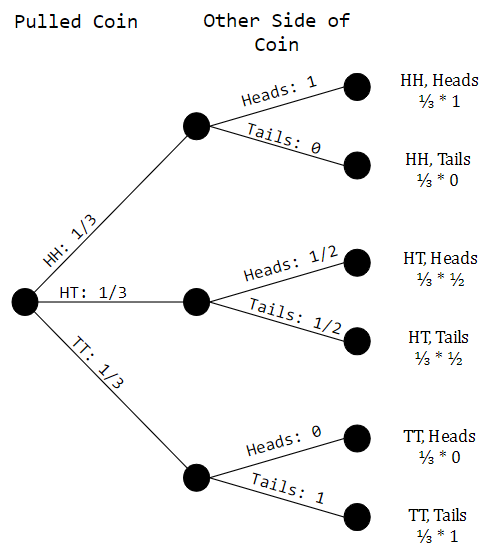
\includegraphics[scale=0.73]{../assets/coin.png}
        \end{center}
        So, we want to find the probability that, given we got heads initially, the otherwise will also have heads. This gives us 
        \[\PR[\text{heads} | \text{got heads}] = \frac{\PR[\text{heads given heads}]}{\PR[\text{got heads}]} = \frac{1/3 \cdot 1}{1/2} = \frac{2}{3}.\]
        Note that one way we can think about getting heads is by thinking about the possible face we \emph{can} get; in this case, we can either get $\{H, H, H, T, T, T\}$. We have a $\frac{3}{6} = \frac{1}{2}$ chance of getting heads. 
    \end{mdframed}
\end{mdframed}

\begin{mdframed}
    (Exercise.) Suppose 80\% of people like peanut butter, 89\% like jelly, and 78\% like both. Given that a randomly sampled person likes peanut butter, what's the probability that they also like jelly?

    \begin{mdframed}
        Let $J$ be the event that someone likes jelly and $B$ be the event that someone likes peanut butter. We know that 
        \[PR[B] = 0.80.\]
        We also know that $\PR[J \cap B] = 0.78$ since 78\% of people like \emph{both} peanut butter and jelly. So, 
        \[\PR[J|B] = \frac{\PR[J \cap B]}{\PR[B]} = \frac{0.78}{0.80} = 0.975.\]
    \end{mdframed}
\end{mdframed}

\begin{mdframed}
    Lupus is a medical phenomenon where antibodies that are supposed to attack foreign cells to prevent infections instead see plasma proteins as foreign bodies, leading to a high risk of blood clotting. It is believed that 2\% of the population suffers from this disease. A test for lupus is 98\% accurate if a person actually has the disease, and 74\% accurate if a person does not have the disease. There is a line from the Fox television show House that is often used after a patient tests positive for lupus: ``It's never lupus.'' Do you think there is truth to this statement? Use appropriate probabilities to support your answer.

    \begin{mdframed}
        Consider the following tree diagram: 
        \begin{center}
            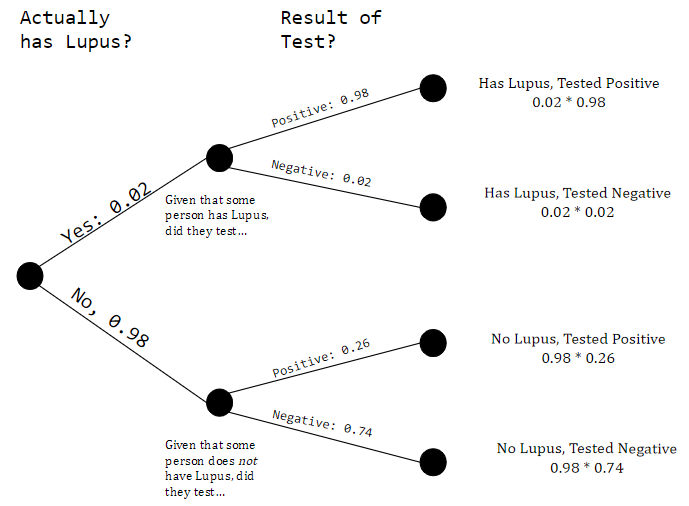
\includegraphics[scale=0.73]{../assets/lupus.png}
        \end{center}
        Then, 
        \[\PR[\text{has lupus} | \text{tested positive}] =\frac{\PR[\text{has lupus + tested positive}]}{\PR[\text{tested positive}]} = \frac{0.02 \cdot 0.98}{0.02 \cdot 0.98 + 0.98 \cdot 0.26} \approx 0.07142.\]
        So, there is some truth to the statement since if someone tests positive for lupus, there's only 7.14\% that they have lupus. 
    \end{mdframed}
\end{mdframed}

\begin{definition}{Independent Events}{10:1}
    Fix a probability space. We say that two events $A$ and $B$ are independent if 
    \[\PR[A \cap B] = \PR[A]\PR[B].\]
\end{definition}
Often, it's convenient to reformulate this definition slightly. In the case that $\PR[B] > 0$, \[\PR[A \cap B] = \PR[A] \PR[B] \iff \frac{\PR[A \cap B]}{\PR[B]} = \PR[A].\] However, notice that \[\frac{\PR[A \cap B]}{\PR[B]} = \PR[A | B]\] so it follows that the independence of $A$ and $B$ is equivalent to asserting that \[\PR[A | B] = \PR[A].\] We could interpret this statement as follows: if $A$ and $B$ are independent, then our confidence in $A$ happening does not change at all even if we're told that $B$ happened (or did not happen). More loosely, knowing whether or not $B$ happens tells us ``nothing'' about whether or not $A$ happenes.

\begin{mdframed}
    (Exercise.) The American Community Survey is an ongoing survey that provides data every year to give communities the current information they need to plan investments and services. The 2010 American Community Survey estimates that 14.6\% of Americans live below the poverty line, 20.7\% speak a language other than English at home, and 4.2\% fall into both categories. Is the event that a randomly chosen American lives below the poverty line independent of the event that the person speaks a language other than English at home?

    \begin{mdframed}
        Define 
        \[\PR[\text{Below Poverty Line}] = 0.146,\]
        \[\PR[\text{Speak Language Other Than English}] = 0.207,\]
        \[\PR[\text{Below Poverty Line AND Speak Language Other Than English}] = 0.042.\]
        Using the formula in (\ref{def:10:1}), notice how \[0.042 \neq 0.146(0.207) = 0.030222.\]
    \end{mdframed}
\end{mdframed}

\begin{mdframed}
    (Exercise.) A bag contains 5 red marbles and 3 blue marbles. Two marbles are drawn randomly from the bag: Alejandra takes the first one and Beatrice takes the second. Is the event that Alejandra's marble is blue independent of the event that Beatrice's marble is blue?

    \begin{mdframed}
        No. If Alejandra takes the first marble and doesn't put it back, then it's possible that she took the blue marble, which affects the probability that Beatrice gets a blue marble.
    \end{mdframed}
\end{mdframed}

\begin{definition}{}{}
    Fix a probability space. Two random variables $X$ and $Y$ are \textbf{independent} if the events $X = a$ and $Y = b$ are independent for all pairs $(a, b)$ where $a$ is a value of $X$ and $b$ a value of $Y$.
\end{definition}


\end{document}